%%%%%%%%%%%%%%%%%%%%%%%%%%%%%%%%%%%%%%%
% Wenneker Resume/CV
% LaTeX Template
% Version 1.1 (19/6/2016)
%
% This template has been downloaded from:
% http://www.LaTeXTemplates.com
%
% Original author:
% Frits Wenneker (http://www.howtotex.com) with extensive modifications by 
% Vel (vel@LaTeXTemplates.com)
%
% License:
% CC BY-NC-SA 3.0 (http://creativecommons.org/licenses/by-nc-sa/3.0/
%
%%%%%%%%%%%%%%%%%%%%%%%%%%%%%%%%%%%%%%

%----------------------------------------------------------------------------------------
%	PACKAGES AND OTHER DOCUMENT CONFIGURATIONS
%----------------------------------------------------------------------------------------

\documentclass[a4paper,12pt]{memoir} % Font and paper size

%%%%%%%%%%%%%%%%%%%%%%%%%%%%%%%%%%%%%%%%%
% Wenneker Resume/CV
% Structure Specification File
% Version 1.1 (19/6/2016)
%
% This file has been downloaded from:
% http://www.LaTeXTemplates.com
%
% Original author:
% Frits Wenneker (http://www.howtotex.com) with extensive modifications by 
% Vel (vel@latextemplates.com)
%
% License:
% CC BY-NC-SA 3.0 (http://creativecommons.org/licenses/by-nc-sa/3.0/)
%
%%%%%%%%%%%%%%%%%%%%%%%%%%%%%%%%%%%%%%%%%

%----------------------------------------------------------------------------------------
%	PACKAGES AND OTHER DOCUMENT CONFIGURATIONS
%----------------------------------------------------------------------------------------

\usepackage{XCharter} % Use the Bitstream Charter font
\usepackage[utf8]{inputenc} % Required for inputting international characters
\usepackage[T1]{fontenc} % Output font encoding for international characters

\usepackage[top=1cm,left=1cm,right=1cm,bottom=1cm]{geometry} % Modify margins

\usepackage{graphicx} % Required for figures

\usepackage{flowfram} % Required for the multi-column layout

\usepackage{url} % URLs

\usepackage[usenames,dvipsnames]{xcolor} % Required for custom colours

\usepackage{tikz} % Required for the horizontal rule

\usepackage{enumitem} % Required for modifying lists
\setlist{noitemsep,nolistsep} % Remove spacing within and around lists

\setlength{\columnsep}{\baselineskip} % Set the spacing between columns

% Define the left frame (sidebar)
\newflowframe{0.2\textwidth}{\textheight}{0pt}{0pt}[left]
\newlength{\LeftMainSep}
\setlength{\LeftMainSep}{0.2\textwidth}
\addtolength{\LeftMainSep}{1\columnsep}
 
% Small static frame for the vertical line
\newstaticframe{1.5pt}{\textheight}{\LeftMainSep}{0pt}
 
% Content of the static frame with the vertical line
\begin{staticcontents}{1}
\hfill
\tikz{\draw[loosely dotted,color=RoyalBlue,line width=1.5pt,yshift=0](0,0) -- (0,\textheight);}
\hfill\mbox{}
\end{staticcontents}
 
% Define the right frame (main body)
\addtolength{\LeftMainSep}{1.5pt}
\addtolength{\LeftMainSep}{1\columnsep}
\newflowframe{0.7\textwidth}{\textheight}{\LeftMainSep}{0pt}[main01]

\pagestyle{empty} % Disable all page numbering

\setlength{\parindent}{0pt} % Stop paragraph indentation

%----------------------------------------------------------------------------------------
%	NEW COMMANDS
%----------------------------------------------------------------------------------------

\newcommand{\userinformation}[1]{\renewcommand{\userinformation}{#1}} % Define a new command for the CV user's information that goes into the left column

\newcommand{\cvheading}[1]{{\Huge\bfseries\color{RoyalBlue} #1} \par\vspace{.6\baselineskip}} % New command for the CV heading
\newcommand{\cvsubheading}[1]{{\Large\bfseries #1} \bigbreak} % New command for the CV subheading

\newcommand{\Sep}{\vspace{1em}} % New command for the spacing between headings
\newcommand{\SmallSep}{\vspace{0.5em}} % New command for the spacing within headings

\newcommand{\aboutme}[2]{ % New command for the about me section
\textbf{\color{RoyalBlue} #1}~~#2\par\Sep
}
	
\newcommand{\CVSection}[1]{ % New command for the headings within sections
{\Large\textbf{#1}}\par
\SmallSep % Used for spacing
}

\newcommand{\CVItem}[2]{ % New command for the item descriptions
\textbf{\color{RoyalBlue} #1}\par
#2
\SmallSep % Used for spacing
}

\newcommand{\bluebullet}{\textcolor{RoyalBlue}{$\circ$}~~} % New command for the blue bullets

 % Include the file specifying document layout and packages

%----------------------------------------------------------------------------------------
%	NAME AND CONTACT INFORMATION 
%----------------------------------------------------------------------------------------

\userinformation{ % Set the content that goes into the sidebar of each page
\begin{flushright}
% Comment out this figure block if you don't want a photo
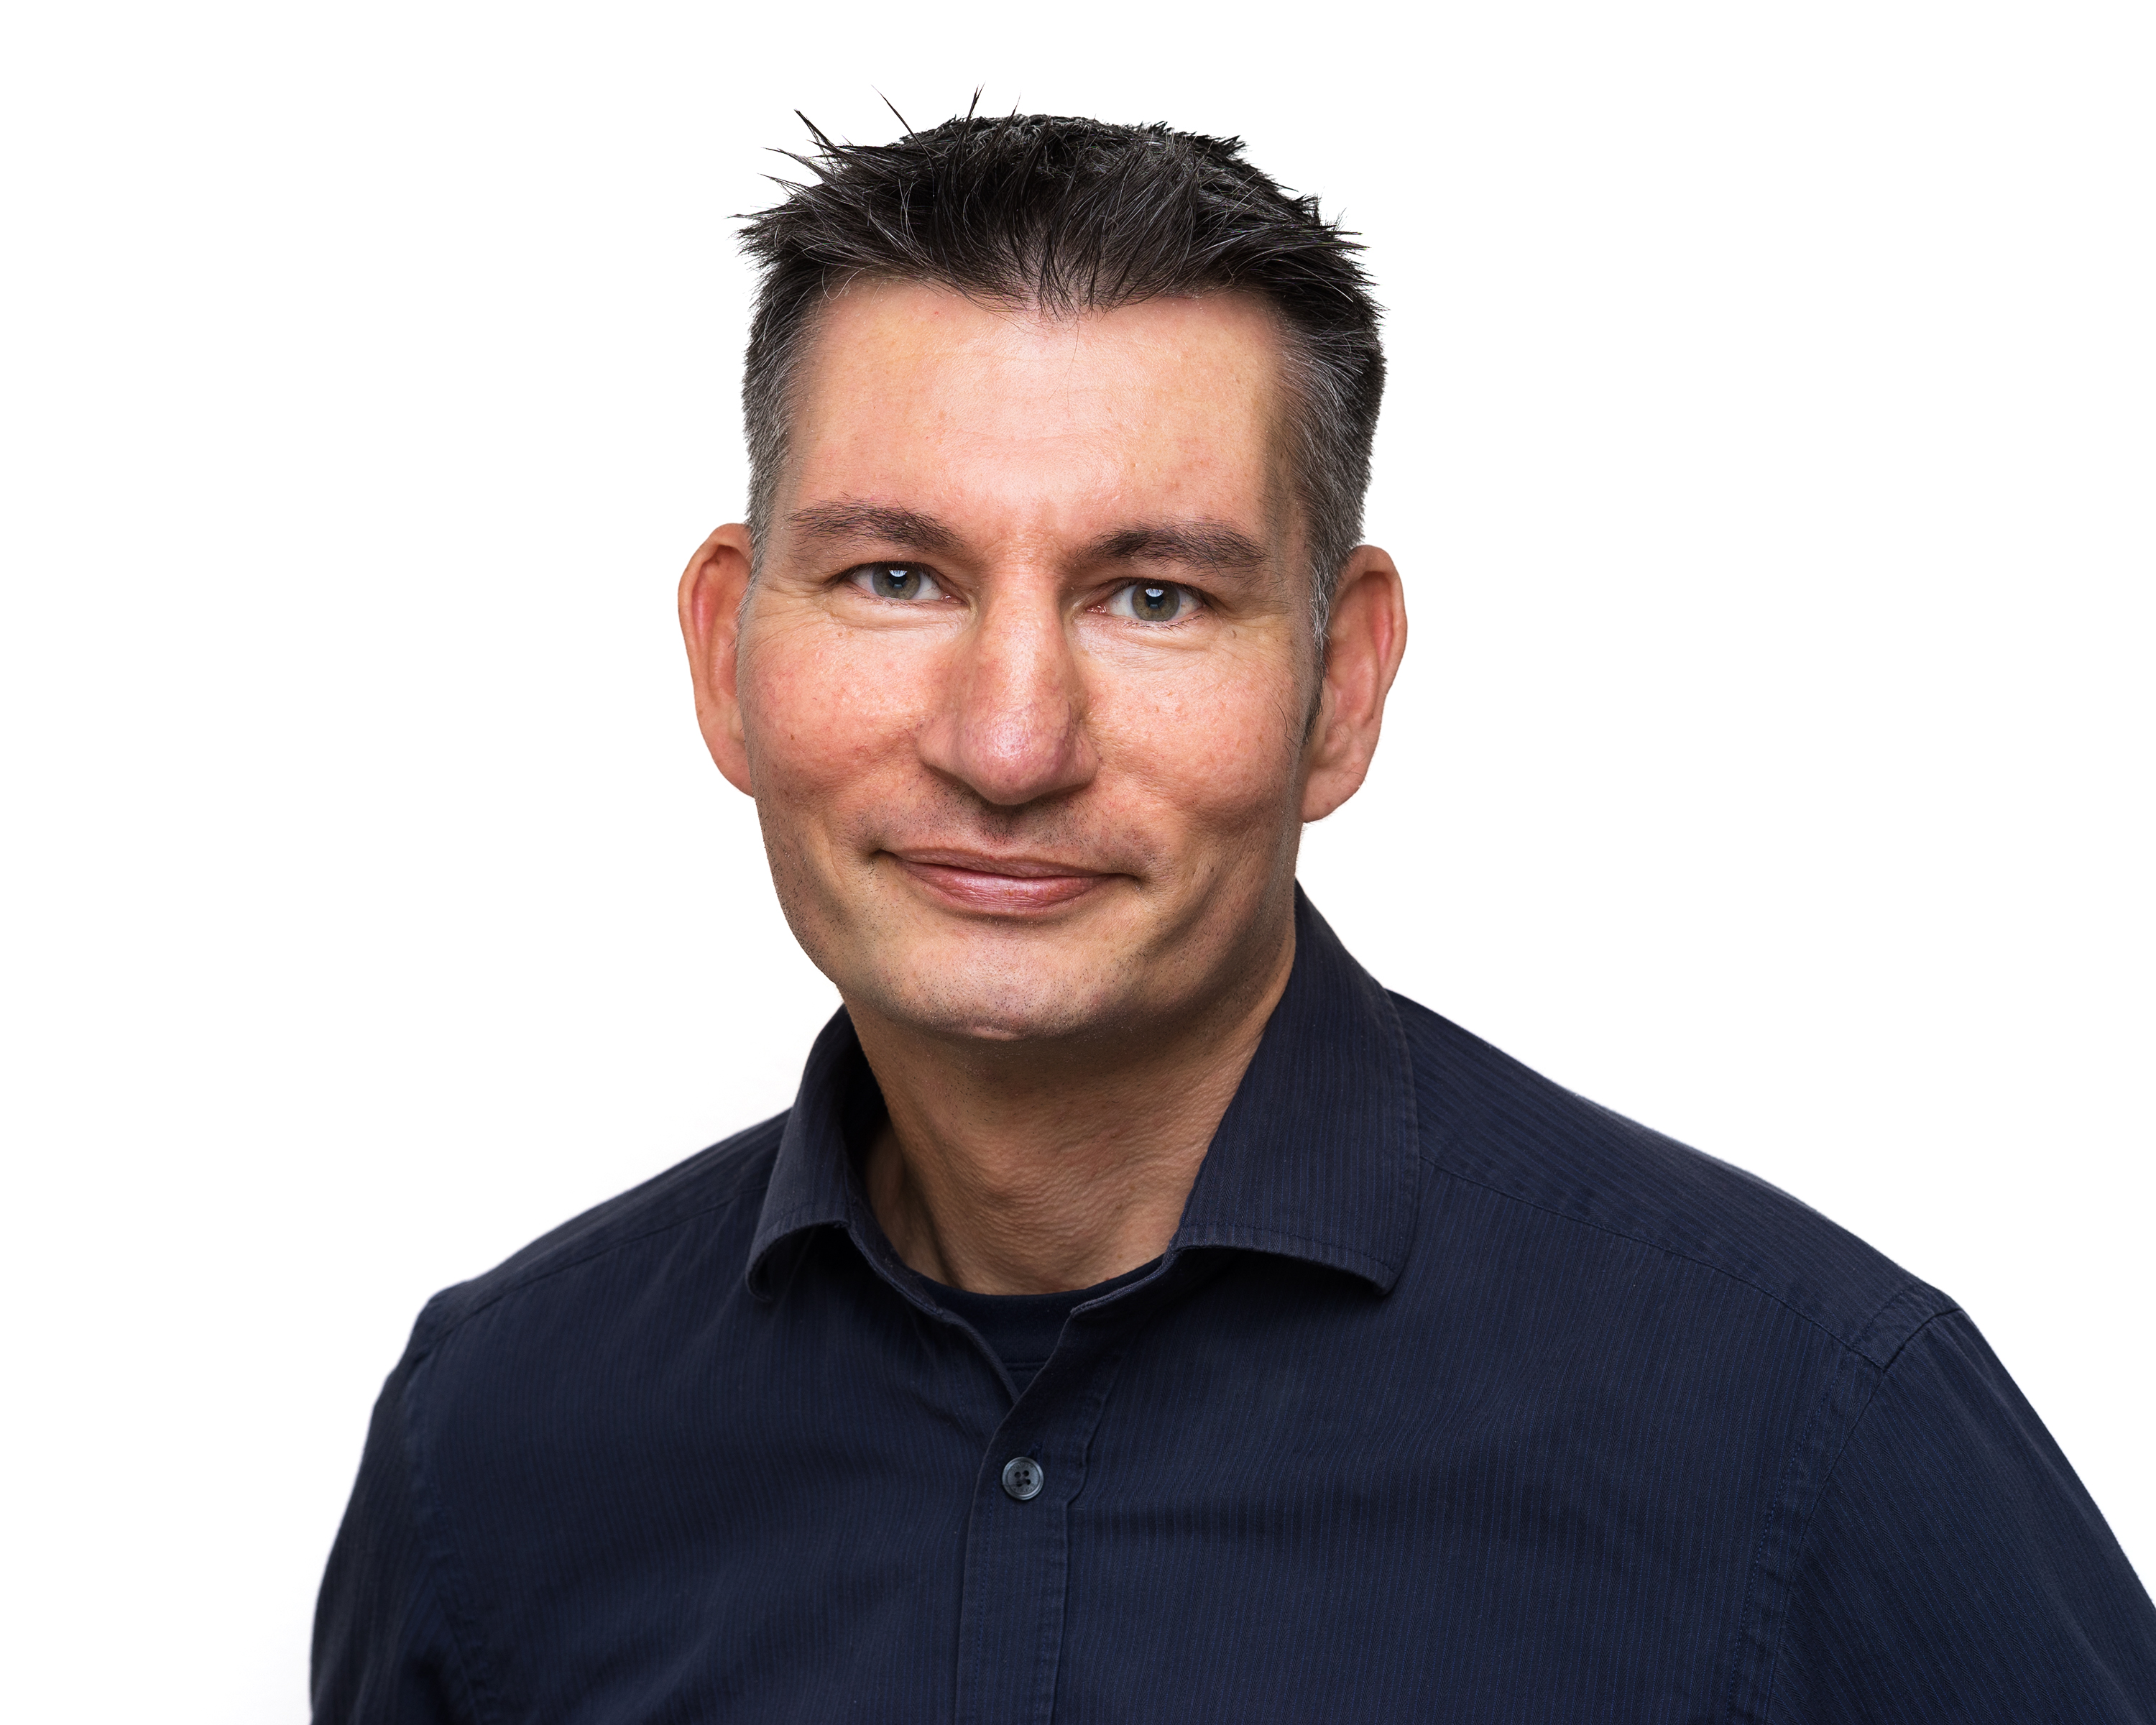
\includegraphics[width=1.0\columnwidth]{photo.jpg}\\[\baselineskip] % Your photo
\small % Smaller font size
Mikael Vatau \\ % Your name
\url{sleepbrunch@gmail.com} \\ % Your email address
+351 926 888 037 \\ % Your phone number
\Sep % Some whitespace
\textbf{Address} \\
Rua Heliodoro 22a \\ % Address 1
Lisbon \\ % Address 2
Portugal \\ % Address 3
\vfill % Whitespace under this block to push it up under the photo
\end{flushright}
}

%----------------------------------------------------------------------------------------

\begin{document}

\userinformation % Print your information in the left column

\framebreak % End of the first column

%----------------------------------------------------------------------------------------
%	HEADING
%----------------------------------------------------------------------------------------

\cvheading{Mikael Vatau} % Large heading - your name

\cvsubheading{Software Engineer} % Subheading - your occupation/specialization

%----------------------------------------------------------------------------------------
%	ABOUT ME
%----------------------------------------------------------------------------------------

\aboutme{About Me}{Eight years experience developing mobile phone platform and
almost 13 year experience in embedded system development both hardware and software. Worked with audio, GPS, touchscreen, Bluetooth,
WLAN and motor control in large and small scaled project. Seven years
experience in customer care.}

%----------------------------------------------------------------------------------------
%	SKILLS
%----------------------------------------------------------------------------------------

\CVSection{Software Development Skills}

%------------------------------------------------

\CVItem{Programming}
{\begin{tabular}{p{0.2\textwidth} p{0.2\textwidth} p{0.2\textwidth}}
\bluebullet C / C++ &  \bluebullet PHP & \bluebullet JS\\
\bluebullet Java &  \bluebullet Shell & \bluebullet Python\\
\end{tabular}}

%------------------------------------------------

\CVItem{Computer Software}
{\begin{tabular}{p{0.2\textwidth} p{0.2\textwidth} p{0.2\textwidth}}
 \bluebullet MySQL &  \bluebullet Linux & \bluebullet Android\\
\end{tabular}}

%----------------------------------------------------------------------------------------
%	EXPERIENCE
%----------------------------------------------------------------------------------------

\Sep % Extra whitespace after the end of a major section
\CVSection{Experience}

%------------------------------------------------
\CVItem{Sep 2017 - Oct 2023, \textit{Technical Support}, Accenture}{
Technical support for Google Adwords and Analytics}

\CVItem{Aug 2016 - Oct 2017, \textit{Customer Support}, CGI Portugal}{Supporting both interal and customer in IT}

\CVItem{Sep 2015 - Aug 2019, \textit{Customer Support}, Teleperformance}{Supporting Swedish customers (Photobox, Boxer)}

\CVItem{Mar 2005 - Apr 2019, \textit{Software Consultant}, Netville AB}{
I was involved in software configuration, low-level audio development, GPS, touch screen, WLAN, Bluetooth, on-site technical support, and application development during my 8-year tenure at Netville:
\begin{itemize}
	\item Camera Web Interface Development (5 months) at Axis Communications for their security cameras.
	\item Platform-Based Applications Development (1 year) at Sony Ericsson: Collaborated on Android applications, such as the calendar, and clock in a small team of 2 that expanded to eight members and 10 applications.
	\item Low-Level Audio Development (2 years) at ST-Ericsson: Involved development for Low Power audio, Wideband Bluetooth, and ALSA, including providing on-site support in Asia and Sweden.
	\item Accessibility App Development (3 months) for Netville Customer: Developed an Android application aiding visually impaired individuals.
	\item Test Software Development (1 year) at Sony Ericsson Mobile Communications AB: to be run on phone to test the GPS signal-to-noise redusing the test time from 30 to 4 seconds.
	\item Configuration Management and Development (4 years) at Ericsson AB: Initially serving as Configuration Manager, later transitioning into a developer role within the Open Platform Architecture department in addition to configuringand supporting PC-lint tool.
\end{itemize}
}

%----------------------------------------------------------------------------------------
%	NEW PAGE DELIMITER
%	Place this block wherever you would like the content of your CV to go onto the next page
%----------------------------------------------------------------------------------------

\clearpage % Start a new page
\userinformation % Print your information in the left column
\framebreak % End of the first column

\CVItem{Jan 2000 - Sep 2004, \textit{Research Engineer}, Robotics Lunds, University}{Worked almost 5 years in multiple hardware and software projects, Maintaining of the departments computer and with development of their website.
\begin{itemize}
	\item Network administration of the departments computers. (IRIX, Linux, and Windows)
	\item Assisted in developing the departments new website (news page and document repository).
	\item Assisted in developing the departments new website (news page and document repository).
	\item Implement, verify and troubleshot controller cards based on 32bit Freescale CPU for DC and Step motor control.
	\item Implement, verify and troubleshot controller cards based on 32bit Freescale CPU for DC and Step motor control.
	\item Hardware and software for controllers to be used in on a robotics arm on attached to a wheelchair (they used the CAN protocoll for communication). 
	\item Worked with an EU project, designing and implementing the controllers and software to be used in bottle openers for physically disabled people. 
\end{itemize}
}


%------------------------------------------------
\Sep % Extra whitespace after the end of a major section
\Sep % Extra whitespace after the end of a major section
%----------------------------------------------------------------------------------------
%	EDUCATION
%----------------------------------------------------------------------------------------

\CVSection{Education}

%Course 2009
\CVItem{2009, SEMC AB (EMEA)}{Linux for Embedded Systems Advanced}

\CVItem{2008, Ericsson AB}{Linux for Embedded Systems}

\CVItem{2006, Ericsson AB}{GPRS Security}

\CVItem{2003, Malmo University}{Practical English in Cross-cultural Communications}

\CVItem{2000, SGI}{IRIX System Administration}

\CVItem{1997 - 2000, Lunds Institute of Technology}{B.Sc.E. Electro Engineer}


\Sep % Extra whitespace after the end of a major section
\Sep % Extra whitespace after the end of a major section

%----------------------------------------------------------------------------------------
%	INTERESTS
%----------------------------------------------------------------------------------------

\CVSection{Interests}

%------------------------------------------------

\CVItem{Professional}{C, Linux, Security, AI}

\CVItem{Personal}{Piano, Chess, Neuroscience}

%------------------------------------------------

\Sep % Extra whitespace after the end of a major section

%----------------------------------------------------------------------------------------

\end{document}

